\chapter{Etude terrain} % 30 pages

	Lors de mon étude terrain, j'ai eu l'occasion de recenser l'avis de nombreuses personnes sur l'open source mais également sur les réflexions menée lors de mon état de l'art.

	Pour cette étude terrain j'ai pu réaliser un sondage de 13 questions autour de ma problématique qui à pu être traité par 38 personnes qui sont lié de près ou de loin à l'open source. Cette étude quantitative me permet de vérifier la véracité de mes hypothèses en cherchant le maximum d'approbation mais aussi de désapprobation de mes idées et réflexions.

	Egalement, l'étude qualitative que j'ai pu réalisé au travers de 4 interviews, m'a permis de confronter mes idées à celles d'autre personnes sensibles au domaine de l'open source . Ceci m'aide à étayer mes réflexions à travers leurs visions.

	J'ai choisi d'orienter mes questionnaires et interviews sur les 4 grands domaines qui représentent selon moi les piliers à batir pour valoriser l'open source, et sur lesquel l'éditeur à la main.

	\section{Plateforme promotrice}

		\subsection{Une interface pour communiquer qui laisse à désirer}

			Autour des plateformes qui contiennent et promouvoie l'open source, sur 31 personnes enregistrées pour cette question, 20 indiquent qu'il y a un manque à palier dans l'interface qui permet de communiquer avec l'éditeur open source. 

			\begin{figure}[ht]
				\center
				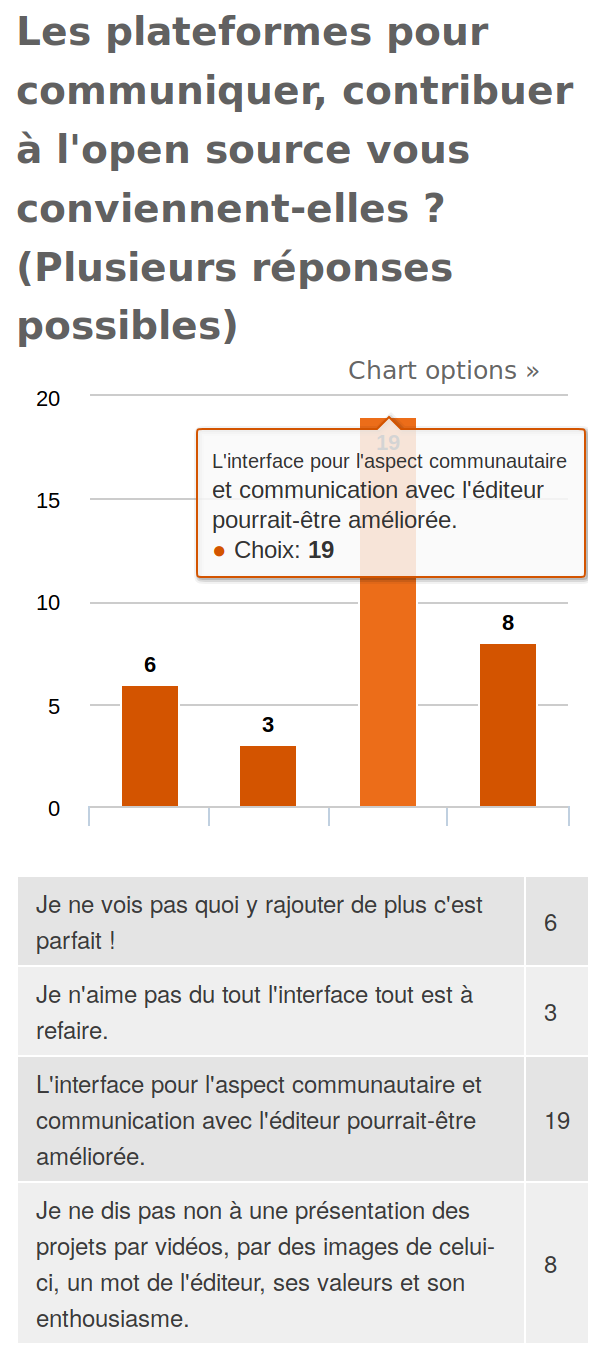
\includegraphics[scale=0.28]{./img/a9}
				\caption{Communication avec l'éditeur}
			\end{figure}

			Il apparait donc que \textbf{la communication qui a un aspect fondamental} pour l'open source \textbf{peux clairement être améliorée} afin de satisfaire non seulement les besoin dans la communication auprès de l'éditeur mais surtout le besoin du consommateur à communiquer correctement.

			Lors de l'interview auprès de Olivier \bsc{Magnial}, ingénieur systèmes embarqués chez l'une des plus grande entreprise promotrice de l'open source : SMILE. Celui-ci à déclaré : 

			\begin{center}
				\textit{
				\textquote{
					Pour \gls{mainliner} du code source, un processus décrit la manière de contribuer, et c'est le plus souvent par mail.(...) Linux, par exemple c'est entièrement du mail, on à des mailing list extrêmement longues et des processus assez carrés !
				}
				}
			\end{center}

			Ainsi même si un moyen de communication et un processus est bien présent pour la contribution. \textbf{Ce n'est pas au travers des plateformes que cette communication pour la contribution est la plus utile}.

			De plus la prise en main d'un logiciel open source est souvent plus compliqué nous révèle Quentin \bsc{Cazelle}, ingénieur logiciel chez Docdoku.\\

			Pourquoi selon lui ?

			\begin{center}
				\textit{
				\textquote{
					Car il y a des fonctionnalités non documentées (...) les plateformes sont incompletes car les développeurs qui contribuent au projets open source ne s'embetent pas à la documentation et a bien expliquer les \gls{issues}
				}
				}
			\end{center}

			J'en déduis donc qu'en plus d'une communication pouvant être amélioré, \textbf{faciliter l'écriture et sensibiliser les consommateurs à l'édition de la documentation} est un axe d'amélioration potentiel.

		\newpage

		\subsection{Un module de présentation}

			Sur la question:

			\begin{center}
				\textit{
				\textquote{
					Les plateformes pour communiquer, contribuer à l'open source vous conviennent-elles ?
				}
				}
			\end{center}

			Seulement 8 personnes sur 31 personnes qui ont répondu à celle-ci sont intéressés pour avoir une présentation sous forme de vidéo du projet, avec un mot de l'éditeur qui communique ses ambitions, ses valeurs.

			\begin{figure}[ht]
				\center
				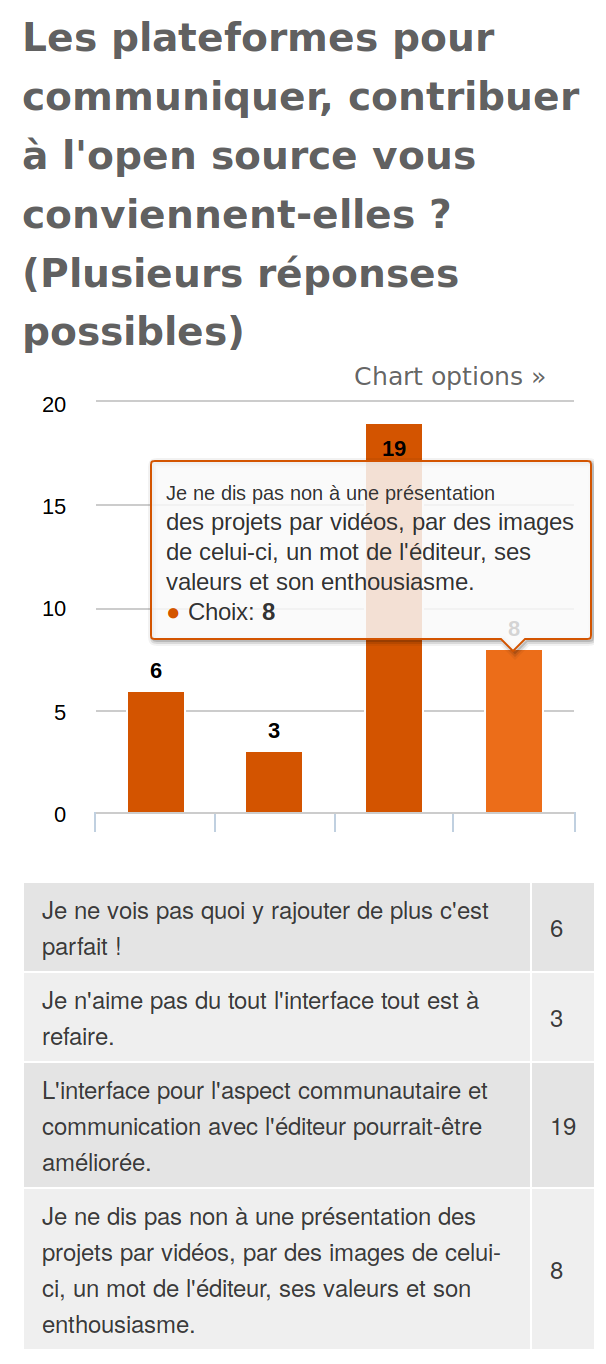
\includegraphics[scale=0.28]{./img/a92}
				\caption{Module de présentation}
			\end{figure}

			Lors de l'interview de Quentin \bsc{Cazelle}, Ingénieur développeur chez Docdoku, celui-ci mentionne tout de même le fait qu'une vitrine à ces plateformes s'impose pour les consommateurs finaux qui ne sont pas développeur.

			\begin{center}
				\textit{
				\textquote{
					La plateforme est un frein pour l'utilisateur final non développeur, il faudrait en effet mettre une vitrine dans un style plus commercial (...)
				}
				}
			\end{center}

			J'en conclus qu'\textbf{une vitrine de présentation du logiciel est bel est bien intéressante} mais \textbf{d'un point de vue utilisateur final} et non développeur contributeur. Ma question dans l'interview ne mentionnais pas la cible de ce module de présentation d'ou le nombres de réponse tout de même favorables à ce module.

		\subsection{Pas d'extrèmes sur les plateformes}

			Très peu de contributeur, c'est-à-dire 6 sur 30, répondent que les plateformes sont parfaites et qu'ils ne voient pas d'amélioration potentielles.

			Il n'y a pas non plus beaucoup d'insatisfait sur celles-ci car seulement 3 ont répondu que toute l'interface était à refaire.

			Je trouve donc que \textbf{les plateformes promotrices sont utilisés et essentielles} à l'open source et ne sont pas à évincer pour l'éditeur.

		\newpage

	\section{Gestion des ressources}

		\subsection{Un mot de l'éditeur pour valoriser la contribution}



		\newpage
	\section{Chez le consommateur}

		\subsection{La contribution du consommateur}

			Dans les personnes interrogés, beaucoup souhaite contribuer ou ont déjà contribué à l'open sources ou souhaitent le faire un jour prochain.60\% y ont déjà contribué, 28\% souhaitent y contribuer un jour.

			\begin{figure}[ht]
				\center
				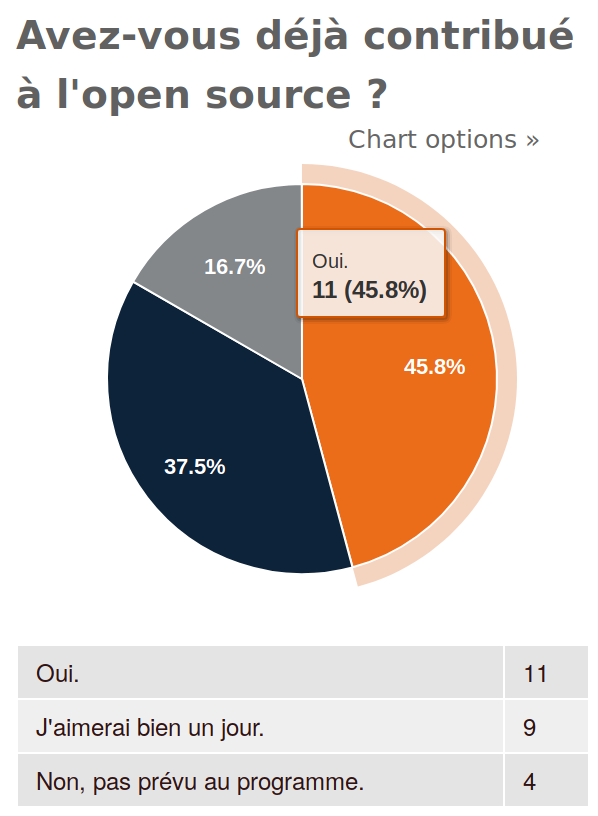
\includegraphics[scale=0.58]{./img/a4}
				\caption{Contribution à l'open source}
			\end{figure}

			L'open source est donc un sujet qui les intéresses et dont \textbf{ils peuvent ou veulent investir du temps en y contribuant}.

			Et ce quelque soit leur domaines d'activité. Sur les 37 personnes qui ont répondu, les domaines d'activités, même si une majoritée est dans l'informatique, sont divers:

			\begin{itemize}[label=\textbullet, font=\LARGE \color{burntorange}]
				\item Edition, Communication, Multimédia
				\item Etude et conseils
				\item Informatique / Télécom
				\item Industriel
				\item Autres
			\end{itemize}

			\begin{figure}[ht]
				\center
				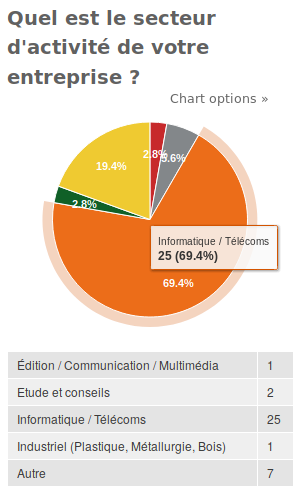
\includegraphics[scale=0.58]{./img/a1}
				\caption{Secteur d'activité des personnes interrogées}
			\end{figure}

			Ainsi \textbf{l'open source n'est pas seulement présent dans l'informatique} et est une préoccupation pour les personnes interrogés.

		\subsection{Le ressenti du consommateur à contribuer}

			J'ai posé une question dans mon questionnaire autour de la perçeption que les gens peuvent avoir dans l'accueil de contribution, s'ils avait des peur ou au contraire qu'il est très agréable de partager avec l'editeur et la communauté ses contributions.

			Globalement, aucun frein n'est ressenti à la contribution et son accueil par l'éditeur, même si ces personnes ne contribuent par pour autant:

			\begin{itemize}[label=\textbullet, font=\LARGE \color{burntorange}]
				\item 46\% des interrogés ont répondu que leurs contribution était très bien accueilli, que l'éditeur et la communauté était agréable.
				\item 43\% Ne prennent pas le temps de contribuer mais n'y vois aucun blocage.
				\item Et seulement 11\% ont peur de contribuer et d'être jugé.
			\end{itemize}

			J'en déduis que la moitiée des personnes ont besoin de \textbf{plus de sensibilisation sur l'importance et les enjeux de la contribution} pour augmenter le nombre de contribution globale.

			Dans leur entreprise, ces personnes considèrent pourtant majoritairement que l'open source est essentiel ou nécessaire.

			Pour 10 personnes, l'open source est essentiel et ils y attachent beaucoup d'importance.
			12 questionnés disent que l'open source est nécessaire dans leur projets. 8 personnes disent que leur entreprise ne s'en soucie pas vraiment et 5 personnes n'ont jamais entendu parlé d'open source dans leur société.

			Ainsi malgré le degré d'importance de l'open source les personnes interrogés n'en font pas une affaire personnelle.

			\begin{figure}[ht]
				\center
				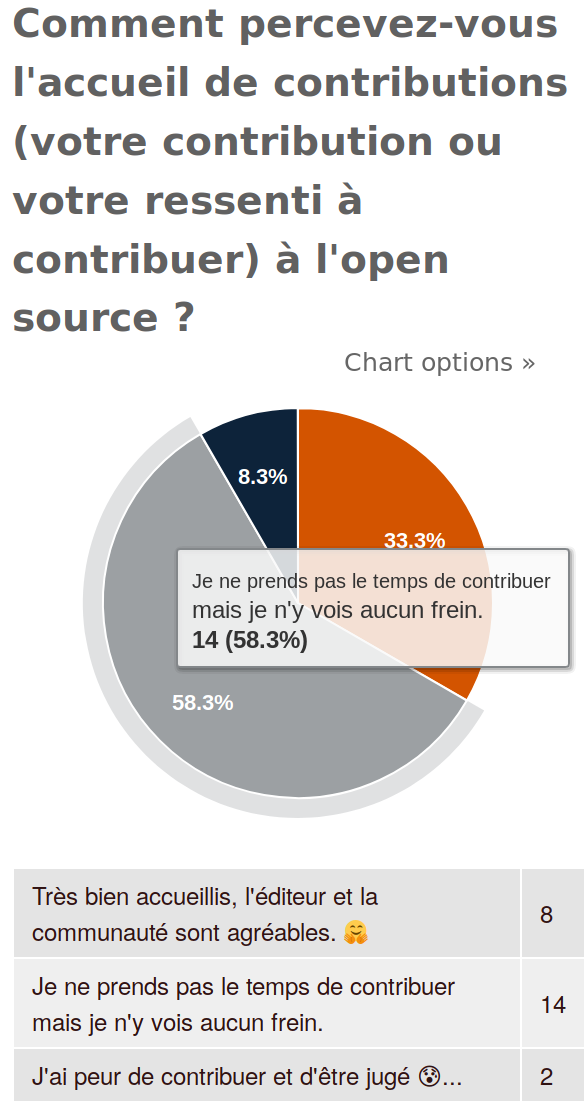
\includegraphics[scale=0.58]{./img/a7}
				\caption{Perception de contribution à l'open source}					
			\end{figure}

			\subsection{Le support payant}

			Dans l'ensemble des personnes interrogés, une forte majorité indiquent qu'ils ne sont pas contre payer du support pour un logiciel open source. 12 personnes ont répondu qu'il était nécessaire et abordable en général. 22 personnes n'ont pas d'objection à payer pour du support logiciel et comprennent qu'il faille rémunérer l'éditeur d'une certaine façon. Et seulement 3 ont répondu qu'il pensait que l'open source devait être gratuit

			\begin{figure}[ht]
				\center
				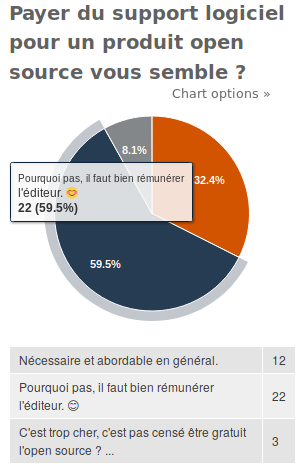
\includegraphics[scale=0.58]{./img/a11}
				\caption{Payer du support logiciel}					
			\end{figure}

			C'est donc que le modèle économique de l'éditeur à travers \textbf{la vente de support logiciel n'est pas un frein à la consommation de l'open source} car beaucoup de personnes interrogées estiment cela comme une moindre chose pour les éditeurs.

		\subsection{Un besoin écouté}

		29 des 37 personnes interrogés ont déclarés qu'après une demande auprès d'un éditeur open source, le besoin du consommateur est suffisemment écouté et ce malgré le fait que les plateformes ne favorisent pas cette communication.

			\begin{figure}[ht]
				\center
				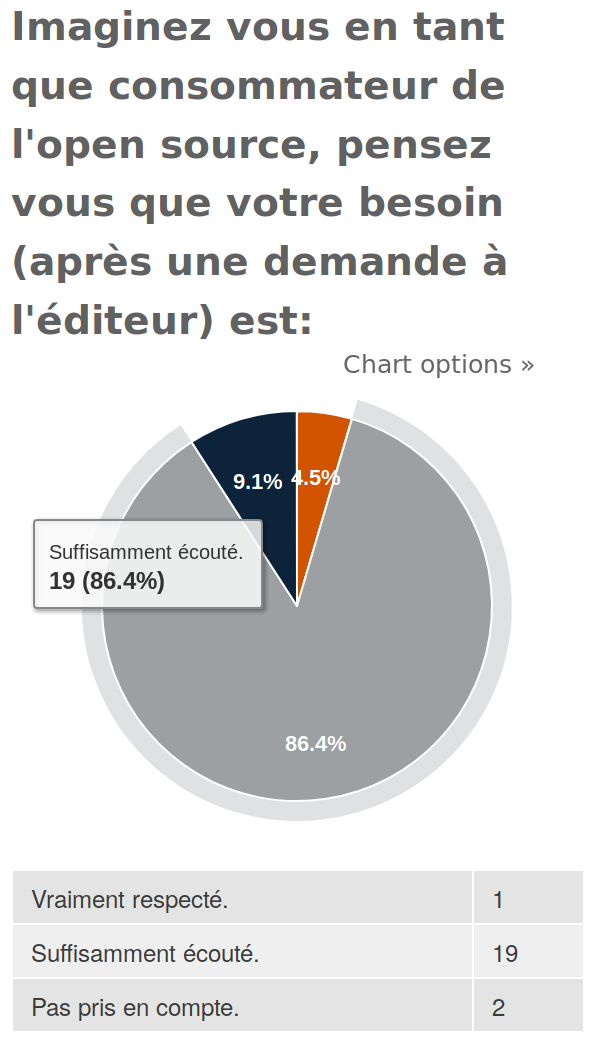
\includegraphics[scale=0.28]{./img/a12}
				\caption{Ecoute du besoin du consommateur}
			\end{figure}

		Ainsi \textbf{la manque de communication dans l'expression du besoin dans l'open source relève d'un problème technique et matériel} plus qu'humain.

	\newpage

	\section{Marketing de l'open source}

		\subsection{L'école et l'open source}

			Sur une 30aine de personnes qui ont répondu à la question: "Devrait on sensibiliser les gens à l'open source dans les écoles informatiques ?", je constate que 12 de ces personnes ont découvert l'open source par le biais de l'école.

			\begin{figure}[ht]
				\center
				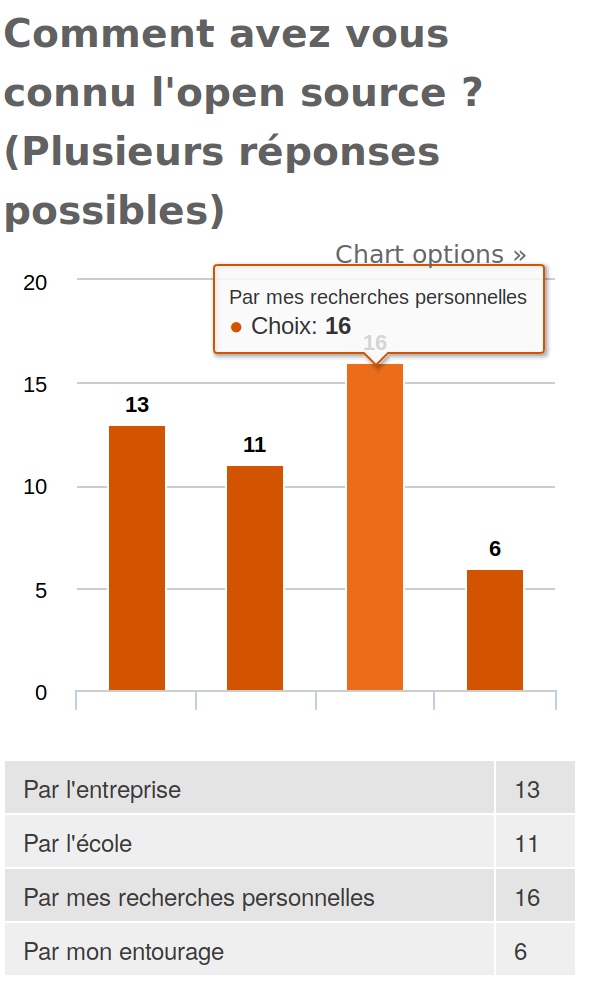
\includegraphics[scale=0.28]{./img/a3}
				\caption{Découverte de l'open source}
			\end{figure}

			Une majoritée des contributeurs, soit 92\% mentionne que l'on devrait bel et bien sensibiliser les gens à l'open source dans les écoles informatiques

			Ceci m'indique que l'enseignement de l'open source dans les école leur à été favorable et qu'ils recommandent donc que le programme contienne un enseignement à l'open source

			Seulement 3 personnes, dont 2 qui ont découvert l'open source à l'école, trouvent que c'est déjà fait intrinsèquement au programme.

			Ainsi \textbf{l'open source est bien un sujet important à traiter au sein de l'école.}

			\begin{figure}[ht]
				\center
				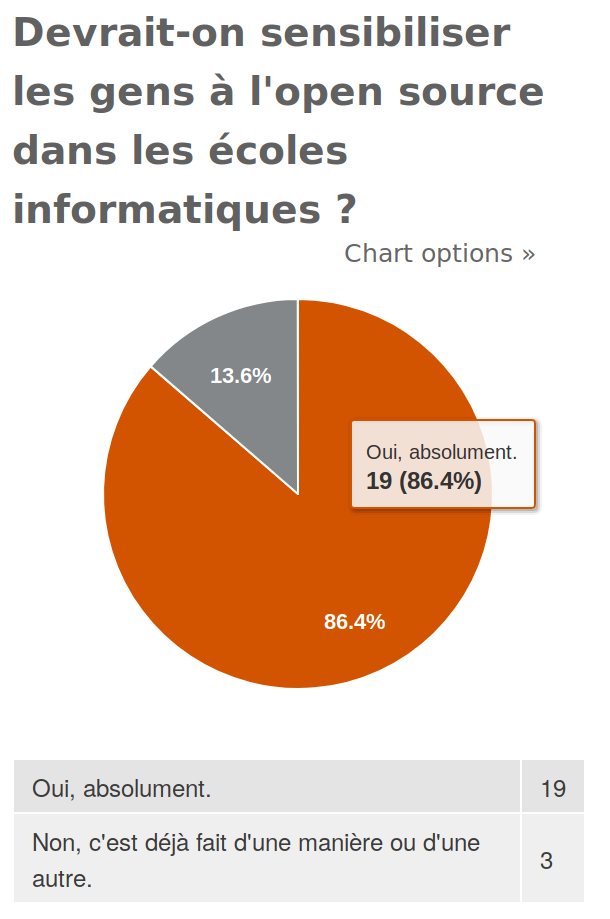
\includegraphics[scale=0.28]{./img/a6}
				\caption{Sensibiliser à l'open source}
			\end{figure}

			A ceci, Quentin \bsc{Cazelle}, qui sort d'une école d'informatique m'indique que son école traitais bien de l'open source et que le sujet était bien présent:

			\begin{center}
				\textit{
				\textquote{
					A l'IUT, j'ai eu des cours sur l'open source, c'était très léger mais on a compris le concept (...) c'est le minimum mais aussi peut-être le maximum que l'on puisse traiter sur ce sujet mais c'est nécessaire. 
				}
				}
			\end{center}

			Il ajoute à cela que l'open source est une brique nécessaire pour le métier de développeur logiciel.

			\begin{center}
				\textit{
				\textquote{
					Quelqu'un qui fait 5 ans d'étude de développeur et ne sait pas ce qu'est l'open source, c'est une abération!
				}
				}
			\end{center}

			Egalement, plus de la moitiée des personnes, soit 21 interrogés ont répondus que l'open source était peu ou tout juste assez évoqué à l'école.

			9 personnes trouvent que les écoles informatiques traitent suffisamment de l'open souce

			Seulement 1 personne à déclaré que l'open source était fortement présent dans les écoles informatiques

			\begin{figure}[ht]
				\center
				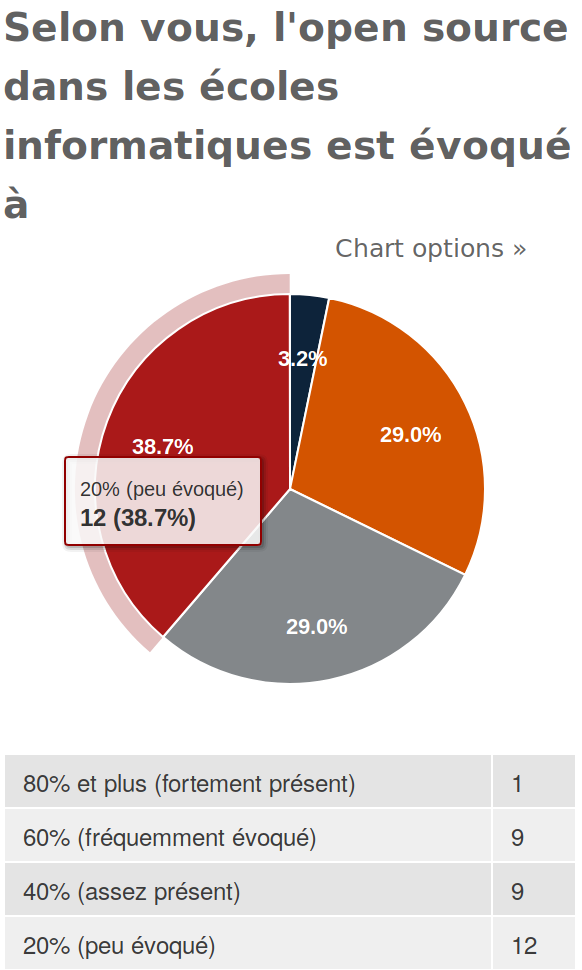
\includegraphics[scale=0.28]{./img/a5}
				\caption{L'open source à l'école}					
			\end{figure}

			J'en conclus que \textbf{ce n'est pas systématique mais l'open source est traité dans les écoles d'informatiques et il se doit de l'être} compte tenu de l'importance qu'il joue pour l'avenir des jeunes diplomés dans leur futures entreprises.









